\iffalse
\def\mytitle{PARALLELOGRAM}
\def\myauthor{Soundarya Naru}
\def\contact{narusoundarya2002@gmail.com}
\def\mymodule{Future Wireless Communication (FWC)}
\documentclass[10pt, a4paper]{article}
\usepackage[a4paper,outer=1.5cm,inner=1.5cm,top=1.75cm,bottom=1.5cm]{geometry}
\twocolumn
\usepackage{setspace}
\doublespacing
\usepackage{graphicx}
\graphicspath{{./images/}}
\usepackage[colorlinks,linkcolor={black},citecolor={blue!80!black},urlcolor={blue!80!black}]{hyperref}
\usepackage[parfill]{parskip}
\usepackage{lmodern}
\usepackage{tikz}
	\usepackage{physics}
%\documentclass[tikz, border=2mm]{standalone}
\usepackage{karnaugh-map}
%\documentclass{article}
\usepackage{tabularx}
\usepackage{circuitikz}
\usetikzlibrary{calc}
\usepackage{amsmath}
\usepackage{amssymb}
\usepackage{physics}
\renewcommand*\familydefault{\sfdefault}
\usepackage{watermark}
\usepackage{lipsum}
\usepackage{xcolor}
\usepackage{listings}
\usepackage{float}
\usepackage{titlesec}
\providecommand{\mtx}[1]{\mathbf{#1}}
\titlespacing{\subsection}{1pt}{\parskip}{3pt}
\titlespacing{\subsubsection}{0pt}{\parskip}{-\parskip}
\titlespacing{\paragraph}{0pt}{\parskip}{\parskip}
\newcommand{\figuremacro}[5]{
    \begin{figure}[H]
        \centering
        \includegraphics[width=0.75\columnwidth]{#2}
        \caption[#3]{\textbf{#3}#4}
        \label{fig:#2}
    \end{figure}
}
\newcommand{\myvec}[1]{\ensuremath{\begin{pmatrix}#1\end{pmatrix}}}
\let\vec\mathbf
\lstset{
frame=single, 
breaklines=true,
columns=fullflexible
}

%\thiswatermark{\centering \put(181,-119.0){\includegraphics[width=0.75\columnwidth]{IIT_logo.png}} }
\title{\mytitle}
\author{\myauthor\hspace{1em}\\\contact\\FWC22012\hspace{6.5em}IITH\hspace{0.5em}\mymodule\hspace{6em}ASSIGN-5}
\date{}
\begin{document}
	\maketitle
	\tableofcontents
   \section{Problem}
   \fi
 In a parallelogram ABCD, $\vec{E}$ and $\vec{F}$ are the
mid-points of sides AB and CD respectively
(see Fig. 
		\ref{fig:9/8/2/5})
Show that the line segments AF
and EC trisect the diagonal BD.

 	\begin{figure}
		\centering
 \includegraphics[width=0.75\columnwidth]{chapters/9/8/2/5/figs/line_1.pdf}
		\caption{}
		\label{fig:9/8/2/5}
  	\end{figure}

	\iffalse

	   % 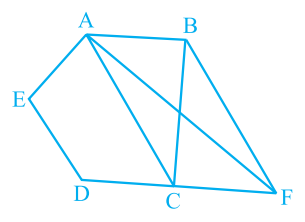
\includegraphics[width=0.75\columnwidth]{diag_1.png}
\begin{center}
   \section{Solution1}

The input parameters for this construction are 
\begin{center}
\begin{tabular}{|c|c|}
	\hline
	\textbf{Symbol}&\textbf{Value}\\
	\hline
	b&6\\
	\hline
	r&5\\
	\hline
	$\theta$&$\frac{\pi}{3}$\\
	\hline
\end{tabular}
\begin{center}
$\vec{A}=\myvec{0\\0}$\\
$\vec{D}=\myvec{r\cos\theta \\ r\sin\theta}$\\
$\vec{B}=\myvec{0\\b}$\\
$\vec{C} = \vec{B}+\vec{C}$\\
\fi
\begin{proof}
From the given information,
	\begin{align}
		\vec{E}=\frac{\vec{A}+\vec{B}}{2}\\
\vec{F}=\frac{\vec{C}+\vec{D}}{2}
	\end{align}
	Hence, 
	\begin{align}
		\vec{E}-\vec{C}&=\frac{\vec{A}-\vec{C}+\vec{B}-\vec{C}}{2}\\
		\vec{A}-\vec{F}&=\frac{\vec{A}-\vec{C}+\vec{A}-\vec{D}}{2}
	\end{align}
	Since $ABCD$ is a parallelogram,
	\begin{align}
		\vec{B}-\vec{C} &= 
	\vec{A}-\vec{D}
	\\
	\implies 
		\vec{E}-\vec{C} &=
\vec{A}-\vec{F}
	\end{align}
	Thus, $AF \parallel EC$.  From Appendix
	  \ref{prop:two-tri-bpt-conv},  using the fact that $\vec{F}$ is the mid point of $CD$, we conclude that $\vec{P}$ is the mid point of $DQ$.  Similarly, it can be shown that $\vec{Q}$ is the mid point of $BP$.
\end{proof}
\iffalse
\end{center}
\end{center}
\textbf{To Prove:} PQ=QB=DP
		\begin{center}
		$\vec{P}=(\vec{2D}+\vec{B})/3$\\
$\vec{Q}=(\vec{2B}+\vec{D})/3$\\
		The distance between P and Q is $\norm{\vec{P}-\vec{Q}}$\\
		The distance between Q and B is $\norm{\vec{Q}-\vec{B}}$\\
		The distance between D and P is $\norm{\vec{D}-\vec{P}}$\\
		if $\norm{\vec{P}-\vec{Q}}$=$\norm{\vec{Q}-\vec{B}}$=$\norm{\vec{D}-\vec{P}}$\\
		then PQ=QB=DP..........(1)\\
		From equation (1) we can say that\\
		 The line segments AF and EC trisect the diagonal BD.\\
		\end{center}
		\section{Solution2}
	 In $\Delta DQC$\\
	 \begin{center}
      F is midpoint of line DC\\
      \end{center}
      \begin{equation}
        	\vec{F}=(\vec{D}+\vec{C})/2
      \end{equation}
       \begin{center}
% $\boldsymbol{FP} \parallel \boldsymbol{QC}$\\
	By converting midpoint theorem \\
	P is mid point of line DQ\\
	\begin{equation}
			\vec{P}=(\vec{D}+\vec{Q})/2
	\end{equation}
			then,\\
			\end{center}
			\begin{center}
			The distance between D and P is $\norm{\vec{D}-\vec{P}}$ \\
			The distance between P and Q is $\norm{\vec{P}-\vec{Q}}$\\
			if $\norm{\vec{D}-\vec{P}}$=$\norm{\vec{P}-\vec{Q}}$ \\
			\end{center}
			\begin{equation}
                DP=PQ 
			\end{equation}
			\begin{center}
			%$\therefore$ AF and EC bisect BD\\
\end{center}						 
	In $\Delta APB$\\
	\begin{center}
	E is midpoint of line AB\\
	\begin{equation}
			\vec{E}=(\vec{A}+\vec{B})/2
			\end{equation}
		  %$\boldsymbol{EQ}\parallel \boldsymbol{AP}$\\
	By converting of mid point theorem\\
		Q is midpoint of BP\\
		\begin{equation}
			\vec{Q}=(\vec{B}+\vec{P})/2
			\end{equation}
			then,\\
	\end{center}
	\begin{center}
	The distance between P and Q is $\norm{\vec{P}-\vec{Q}}$\\
	The distance between Q and B is $\norm{\vec{Q}-\vec{B}}$\\
	if $\norm{\vec{P}-\vec{Q}}$=$\norm{\vec{Q}-\vec{B}}$\\
	\end{center}
	\begin{equation}
	PQ=QB
	\end{equation}
	\begin{center}
	$\norm{\vec{D}-\vec{P}}$=$\norm{\vec{P}-\vec{Q}}$=$\norm{\vec{Q}-\vec{B}}$\\
$\therefore$ from (5),(8) \\
\begin{equation}
DP=PQ=QB
\end{equation}	
		from equation (9) we can say that the \\	
	 The line segments AF and EC trisect the diagonal BD.\\
	 AF and EC trisect BD.
	\end{center}
The below python code realizes the above construction:	\\
\begin{lstlisting}
https://github.com/soundaryanaru/FWC-assignments/tree/main/Matrix/Line_assignment/code
\end{lstlisting}
 
\section{Construction}
\includegraphics[width=0.75\columnwidth]{line_1.pdf}
 	
\bibliographystyle{ieeetr}
\end{document}
\fi
